% !Mode:: "TeX:UTF-8"

\chapter{公司概况}{in}
\label{chap01}

\section{公司基本情况}{}
中恒通(福建)机械制造有限公司正式成立于2008年3月24日,由两位发起人卢汉达、张芳辉共同出资组建,公司注册资本为6300万元,经报武平县工商行政管理局,注册号:3508 2410 0002 276,经由变更股东程序,当前公司法定代表人为卢文煊。目前公司的主营业务为商用车制动鼓、轮毂、铸钢和冲焊驱动桥壳、工程机械桥壳、平衡悬架总成、刹车盘、刹车片等载重汽车底盘零部件的生产与销售,生产的「中恒通」牌系列产品通过「ISO/TS16949:2009」质量体系认证。

\subsection{股本结构}{}

截止2013年9月11日,公司的股本结构如下:
%%------------------------------------------------------------------------
  \begin{center}
  \begin{threeparttable}\vspace{-1.0cm}
  %%
 %\caption{股本构成}
 \renewcommand{\arraystretch}{1.1} \arrayrulewidth=0.8pt \tabcolsep=8pt
 	 \begin{tabular}{cccrr}
 	 &&&& {\small 单位:元}\\
	\hline\hline
\rowcolor{mycyan}	股东名称 	& 股东性质 & 出资方式 &  出资金额      & 持股比例  \\
	\hline \renewcommand{\arraystretch}{1}
	卢汉旺   & 国内自然人 & 货币    &  57,330,000 &  91\% \\
	张芳辉   & 国内自然人 & 货币    &   5,670,000 &  9\% \\ 
	\bottomrule
	\end{tabular}
\end{threeparttable}
\end{center}
%%------------------------------------------------------------------------
\subsection{组织结构}{}
公司于2010年3月9日进行股权变更登记,并于同年4月8日更新依据新修改的公司章程而设立的组织结构。目前,公司法定代表人为卢文煊,管理层组织架构为
\begin{compactitem}
\item 董事长:卢汉旺
\item 副董事长:张芳辉
\item 董事:钟添臣
\item 监事:赖加森
\item 经理:卢文煊 
\end{compactitem}
%%-----------------------------------------------------------------------
 %------------------------------------------------------
  \begin{figure}%[!h]
   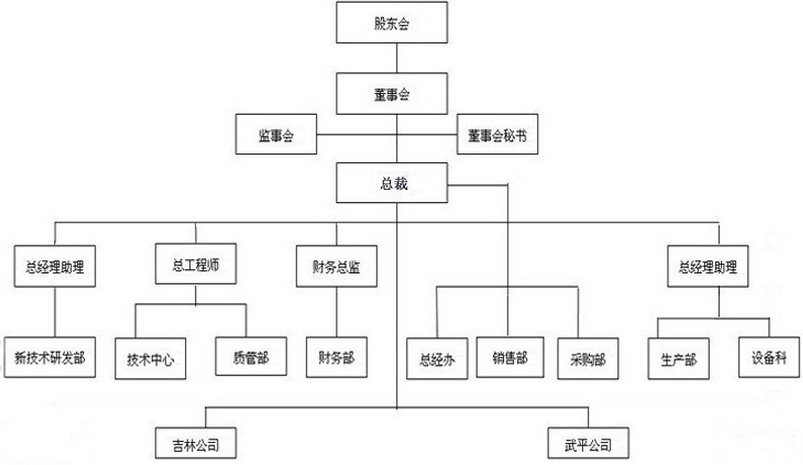
\includegraphics[width=15cm,height=10cm]{figures/org}
   \caption{中恒通组织结构图:{\footnotesize 资料来源:公司介绍}}
  \end{figure}
 %------------------------------------------------------
 
\section{公司经营与财务情况}{}
%%------------------------------------------------------------------------
\subsection{经营情况}{}

中恒通公司的主要营业范围:工程机械、矿山机械、汽车配件、待机机械产品的生产与销售服务。其目前的主要营收来自汽车底盘部件,未来在其他相关行业有待发展。下表给出了该公司的主要营业状况。公司在本年度内总资产增加了34 894千元,增加幅度为9.46\%,主要是由于所有者权益的大幅提高,导致公司为分配利润增加了33 037千元。这表明公司在过去的一个会计年度内业绩表现良好,整体经营取得显著提高。由于主营业务的强劲发展(24.15\%),其利润总额增长了14 257千元,增加幅度为48.14\%。
%%------------------------------------------------------------------------
  \begin{center}
  \begin{threeparttable}\vspace{-1.0cm}
  %%
 \caption{主要经营指标}
 \renewcommand{\arraystretch}{1.1} \arrayrulewidth=0.8pt \tabcolsep=8pt
 	 \begin{tabular}{crrrc}
 	 &&&& {\small 单位:元}\\
	\hline\hline
\rowcolor{mycyan}	\bfseries 项目 	& \bfseries 2013年度\hspace{1em} & \bfseries 2012年度\hspace{1em} &  \bfseries 增减额\hspace{1.5em}      & \bfseries 增减($\%$)  \\
	\hline \renewcommand{\arraystretch}{1}
	总资产	& 403,747,108.06	& 368,852,226.45	& 34,894,881.61	& 9.46 \\
	负债总额	& 157,172,080.45	& 159,079,371.06	& -1,907,290.61	& -0.01\\
	所有者权益	& 246,575,027.61	& 209,772,855.39	& 36,802,172.22	& 17.54\\
	\midrule
	主营收入 & 402,880,199.53 & 324,498,460.53    &  78,381,739.00 &  24.15 \\
	主营利润 & 71,592,206.36 & 55,845,432.62    &   15,746,773.74 &  28.20 \\
	营业利润 & 38,000,711.07 &	29,615,752.56 &	8,384,958.51 &	28.31\\
	利润总额 & 43,873,186.11 &	29,615,752.56 &	14,257,433.55 &	48.14 \\
	\bottomrule
	\end{tabular}
\end{threeparttable}
\end{center}
%%------------------------------------------------------------------------

\subsection{财务情况}{}
根据现有企业年度会计报表资料,我们将部分重要财务指标罗列如下,具体财务分析将在下一章节分析。从对公司的偿债能力分析,公司的资产负债率进一步降低,减少幅度为12.67\%。对于债券人来说,公司的资产负债率表明公司的债务负担程度,该比率越低,其总体偿还债务的能力越强,即债权人的权益得到保证的程度越高。从短期资金流动性上看,公司的流动比率为1.3,速动比率0.95,说明公司在短期内的资金流动性较为薄弱,提醒投资者关注公司在近期的现金流变动情况。

在投资收益方面,公司本年度内总资产报酬率为10.87\%,同比上升了35.34\%,表明公司在盈利创收方面表现强劲;其息税前利润率为10.89\%,增加幅度19.32\%。以上数据说明公司的投资回报率较为突出,涨幅强劲。
%%------------------------------------------------------------------------
  \begin{center}
  \begin{threeparttable}\vspace{-1.0cm}
  %%
 \caption{主要财务指标}
 \renewcommand{\arraystretch}{1.1} \arrayrulewidth=0.8pt \tabcolsep=8pt
 	 \begin{tabular}{crrrc}
 	 % &&&& {\small 单位:元}\\
	\hline\hline
\rowcolor{mycyan}	\bfseries 项目 	& \bfseries 2013年度 & \bfseries 2012年度 &  \bfseries 增减额      & \bfseries 增减($\%$)  \\
	\hline \renewcommand{\arraystretch}{1}
	资产负债率 & 38.93 & 43.13 & -5.47 & -12.67\\
	流动比率 & 1.30 & 0.94 & 0.37 & 39.20\\
	速动比率 & 0.95 & 0.61 & 0.35 & 57.29\\
	现金比率 & 16.10 & 15.17 & 0.93 & 6.16\\
	股东权益比率 & 61.07 & 56.87 & 4.20 & 7.38\\
	\midrule
	总资产报酬率 & 10.87 & 8.03 & 2.84 & 35.34\\
	净资产收益率 & 15.27 & 10.59 & 4.68 & 44.21\\
	息税前利润率 & 10.89 & 9.13 & 1.76 & 19.32\\
	%经营性现金流量净额 & 3,140,380.63 & 50,813,148.61 & -47,672,767.98 & -93.82 \\	
	\bottomrule
	\end{tabular}
\end{threeparttable}
\end{center}
%%------------------------------------------------------------------------

